\documentclass[10pt]{article}
\usepackage[utf8]{inputenc}
\usepackage{kotex}
\usepackage{graphicx}
\usepackage{subfigure}
\usepackage{titling}
\setlength{\droptitle}{-2cm}
\usepackage{array}
\usepackage{amssymb}
\usepackage{amsmath}
\usepackage{siunitx} 
\usepackage{enumerate} 
\usepackage{pgfplots}
\usepackage{pgfplotstable}
\usepackage{tikz,pgfplots}
\usepackage{wasysym}
\usepackage{geometry}
\usepackage{authblk}
\usepackage{kotex}
\usepackage{bibunits}
\usepackage{tabularx}
\usepackage{hyperref}
\usepackage{pythonhighlight}

\geometry{
    a4paper,
    total={170mm,257mm},
    left=20mm,
    top=20mm,
}

\title{\textbf{Mathematical Foundation of DNN : HW 1}}
\author{Jeong Min Lee}

\begin{document}
\maketitle

\section{}
In this problem, I followed the notation given by the Petersen and Pedersen\cite{Petersen2008}. Also, I denote the element of matrix $X$ in $i$th row and $j$th column as $X_{ij}$
\subsection*{a}
\begin{align} 
    \left({\partial \over \partial \theta} l_i(\theta)\right)_j &= {\partial l_i \left(\theta\right)\over \partial \theta_j} \\
    &= (X_i^T\theta - Y) X_{ij}
\end{align}

By enumberating the last equation in column vector, one can get the following result.

\begin{equation}
    {\partial \over \partial \theta} l_i(\theta) = (X_i^T\theta - Y_i)X_i
\end{equation}
Note that $(X_i^T\theta - Y_i)\in \mathbb{R}$ and thus, enumeration affects only to the last $X_{ij}$. (It results in $X_i$) 

\subsection*{b}
\begin{align}
    \mathcal{L}(\theta) &= \frac{1}{2} \lVert X\theta - Y \rVert^2 \\ &= \frac{1}{2}\sum_i \left(X_i^T\theta - Y_i\right)^2 \\ &= \sum_i l_i(\theta)    
\end{align}

From the obseravtion above and the result of the problem(a),

\begin{align}
    \nabla_\theta \mathcal{L}(\theta) &= \sum_i \nabla_\theta l_i(\theta) \\ &= \sum_i (X_i^T\theta - Y_i)X_i \\ &= \sum_i X_i^T\theta X_i - X_i Y_i
\end{align}

According to the hint given by the original problem statement, noting that the matrix consisting of the $X_i$ as a column is $X^T$,

\begin{align}
    \nabla_\theta \mathcal{L}(\theta) &= X^T \begin{pmatrix} X_1^T\theta \\ X_2^T\theta \\ \vdots \\ X_N^T\theta\end{pmatrix} - X^TY \\
    &= X^T\begin{pmatrix} X_1^T \\ X_2^T \\ \vdots \\ X_N^T\end{pmatrix}\theta - X^TY \\ &= X^TX\theta - X^TY \\ &= X^T(X\theta - Y) 
\end{align}


\section{}

Since $f'(\theta) = \theta$, 
\begin{align}
    \theta^{(k+1)} &= \theta^{(k)} - \alpha f^\prime(\theta^{(k)}) 
    \\ &= (1-\alpha) \theta^{(k)}
\end{align}
\footnote{To resolve the confusion due to the notation between $k$th element and power of $k$, I used parenthesis to denote the $k$th element}

\begin{align}
    &\frac{\theta^{(k+1)}}{\theta^{(k)}} = 1-\alpha \\
    &\therefore \theta^{(k)} = \theta^{(0)}(1-\alpha)^k
\end{align}

If $\alpha >2$, then $\left|1-\alpha\right|>1$. This results in $\theta^{(k)} \rightarrow \infty $ as $k\rightarrow \infty$
\section{}

From problem 1, I showed the following. 

\begin{equation}
    \nabla f(\theta) = X^T(X\theta - Y)
\end{equation}
Inserting it to the GD,

\begin{align}
    \theta^{(k+1)} &= \theta^{(k)}  - \alpha X^T(X\theta^{(k)}- Y) \\
    &= \theta^{(k)} - \alpha X^TX\theta^{(k)} + \alpha X^TY \\
    &= \theta^{(k)} - \alpha X^TX\theta^{(k)} + \alpha XX^T \theta^\star
\end{align}
By substracting $\theta^\star$ on both side of equation 21, the following equation is derived.

\begin{equation}
    \theta^{(k+1)} - \theta^\star = (I_p - \alpha X^TX)(\theta^{(k)} - \theta^\star)
\end{equation}

Note that $I_p$ denotes identity matrix whose dimension is $p \times p$. This recursive equation has the following closed form. Here I denoted $\theta^{k} - \theta^{\star}$ as $\zeta^{(k)}$.

\begin{equation}
    \zeta^{k} = \zeta^{(0)}(I_p - \alpha X^TX) 
\end{equation}

According to SVD, 
\begin{equation}
    X^TX = V\Sigma^2V^T
\end{equation}
where $V \in O(p)$. I assumed that diagonal entries of $\Sigma^2 = \text{diag}(\sigma_1^2, \sigma_2^2, \cdots, \sigma_p^2)$, the eigenvalues of $X^TX$ are ordered. 
This implies that $\rho(X^TX) = \sigma_1^2$. Since $V \in O(p)$, the equation 23 can be written as follows.

\begin{align}
    \zeta^{k} &= \left(VI_pV^T - \alpha V\Sigma^2V^T\right)^k\zeta^{(0)} \\
    &= V(I_p - \alpha \Sigma^2)^kV^T \zeta^{(0)}
\end{align}

\begin{align}
    \lVert\zeta^{(k)}\rVert^2 &= [\zeta^{(0)}]^TV^T (I_p - \alpha\Sigma^2)^{2k}V\zeta^{(0)} \\
    &= [\zeta^{(0)}]^TV^T \text{diag}(1 - \alpha \sigma_1^2, 1 - \alpha \sigma_2^2, \cdots. 1 - \alpha \sigma_p^2)^{2k} V\zeta^{(0)} \\
    &= [\zeta^{(0)}]^TV^T \text{diag}((1-\alpha \sigma_1^2)^{2k}, (1-\alpha \sigma_2^2)^{2k}, \cdots, (1-\alpha \sigma_p^2)^{2k})
\end{align}

Since $\alpha > 2/\rho(X^TX)$ implies $\left|1-\alpha \sigma_1^2\right|>1$, $\zeta^{(k)}$ diverges, that is $\theta^{(k)}$.



\section{}
\begin{figure}[!h]
    \begin{center}
        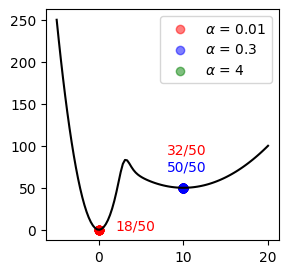
\includegraphics{Fig1.png}
        \caption{The result of gradient descent of $f(x)$ is described. The proportion of initial points that converges to each local minimum is depicted. The color of given ratio matches to the each $\alpha$. Note that there is no scatter in this plot corresponding to $\alpha = 4$ since none of them converged. }
    \end{center}
\end{figure}

I implement my own gradient descent algorithm to solve this problem. As mentioned in homework document, I use three learning rate $\alpha = [0.01,0.3,4]$. Furthermore,
for the robust analysis, I randomly sampled 50 initial point of x for each $\alpha$. This result agrees to the general notion that GD with small learning rate temps to converge both of local minma, while that with intermediate learning rate converges only to the wide local minimum. 
The following python code is the code used to solve this problem.

\begin{python}
import numpy as np
import matplotlib.pyplot as plt
alpha_lst = [0.01, 0.3,4]
iter_num = 50 # number of sampling
epsilon = 1e-4 # acceptable level
result = dict() # contain the result of experiment
max_step = 1000 # maximum step not to run while loop infintely

for alpha in alpha_lst:
    print(f"--------------------------alpha = {alpha}---------------------------------------")
    result[alpha] = []
    for i in range(iter_num):
        x = 25*np.random.random_sample()-5
        x_init = x
        step = 0
        while fprime(x) > epsilon or step < max_step:
            print(f"step : {step}/{max_step}")
            step +=1
            x = x - alpha * fprime(x)
        result[alpha].append((x,x_init))
\end{python}
\section{}
Since there is no theoretical analysis requirment on this probelm. I briefly introduce my code. The following code box is the code I implemented. 

\begin{python}
    import numpy as np

    class Convolution1d :
        def __init__(self, filt) :
            self.__filt = filt
            self.__r = filt.size
            self.T = TransposedConvolution1d(self.__filt)

        def __matmul__(self, vector) :
            r, n = self.__r, vector.size
            
            return np.asarray([sum([self.__filt[i] * vector[i+j] for i in range(r)]) for j in range(n-r+1)])  # IMPLEMENT THIS
        
    class TransposedConvolution1d :
        '''
        Transpose of 1-dimensional convolution operator used for the 
        transpose-convolution operation A.T@(...)
        '''
        def __init__(self, filt) :
            self.__filt = filt
            self.__r = filt.size

        def __matmul__(self, vector) :
            r = self.__r
            n = vector.size + r - 1
            vector = np.concatenate([np.zeros((r-1,)), vector, np.zeros((r-1,))]) # padding
            return  np.asarray([sum(self.__filt[::-1] * vector[i:i+3]) for i in range(len(vector)-r+1)]) # IMPLEMENT THIS

    def huber_loss(x) :
        return np.sum( (1/2)*(x**2)*(np.abs(x)<=1) + (np.sign(x)*x-1/2)*(np.abs(x)>1) )
    def huber_grad(x) :
        return x*(np.abs(x)<=1) + np.sign(x)*(np.abs(x)>1)


    r, n, lam = 3, 20, 0.1

    np.random.seed(0)
    k = np.random.randn(r)
    b = np.random.randn(n-r+1)
    A = Convolution1d(k)
    #from scipy.linalg import circulant
    #A = circulant(np.concatenate((np.flip(k),np.zeros(n-r))))[r-1:,:]


    x = np.zeros(n)
    alpha = 0.01
    for _ in range(100) :
        x = x - alpha*(A.T@(huber_grad(A@x-b))+lam*x)

    print(huber_loss(A@x-b)+0.5*lam*np.linalg.norm(x)**2)
\end{python}

For \textbf{Convolution1d.\_\_matmul\_\_()}, I implemented it by using simple list comprehension. $i$th iteration calculate the product of each elements in $k$ and $v$ and \textbf{sum()} function, python native function, calcaulate their sum.
This repeat until the every row of $A$ is seen. Hoever, for \textbf{TransposeConvlution1d.\_\_matmul()\_\_}, I padded the target vector. I strongly believe implementing this function in list comprehension with single line is possible, but 
I think it is not that intuitive to read. Thus, to maintain the readability of my code, I add additional single line that pad zeros on the target vector. 
\bibliographystyle{unsrt}
\bibliography{ref.bib}
\end{document}